%--------------------------------------------------------------------------------
%----------------------------------------------------------------------
\section{Design and implementation}\label{sec:design}
This section gives more detailed information about the design of GreenMirror and some details of its implementation. GreenMirror is written with version 8 of the Java Runtime Environment and developed under Eclipse Luna. It highly depends on the integrated JavaFX library and uses JUnit \cite{junit} for testing, JOpt Simple \cite{joptsimple} for handling the command line options (see \cref{sec:design;sub:detailedwf}), Groovy \cite{groovy} (see \cref{sec:design;sub:interface}) for its JSON implementation and scripting capabilities and the Eclipse JDT annotation package for using \lstinline{NonNull} annotations. GreenMirror is composed of 114 classes in 12 packages, which sums up to a total of 7429 lines of code.
%--------------------------------------------------------------------------------
\subsection{Package structure}\label{sec:design;sub:package}
GreenMirror's package structure is fairly self-evident. Still, a short explanation per package is in place. Details about how to extend certain subpackages are available in \cref{app:ext}. Corresponding class diagrams depicting all relations between the classes are unfortunately too large to be a useful addition to this report, although they are available on the repository.
\begin{description}
\item[\texttt{greenmirror}] is the main package containing classes shared by the client and server.
\item[\texttt{greenmirror.client}] contains all classes that pertain solely to the client.
\item[\texttt{greenmirror.client.modelinitializers}] contains all implemented model initializers that can be used by the client. See \cref{sec:design;sub:interface}.
\item[\texttt{greenmirror.client.traceselectors}] contains all implemented trace selectors that can be used by the client. See \cref{sec:design;sub:interface}.
\item[\texttt{greenmirror.commandlineoptionhandlers}] contains all command line option handlers, both for the client and the server. The \lstinline{@ClientSide} and \lstinline{@ServerSide} annotations indicate where they are used. See \cref{sec:design;sub:detailedwf}.
\item[\texttt{greenmirror.commands}] contains all commands that are sent from the client to the server and vice versa. It also contains all handlers that interpret and handle received commands. The handlers have \lstinline{@ClientSide} and \lstinline{@ServerSide} annotations to indicate where their respective commands are received.
\item[\texttt{greenmirror.fxpropertywrappers}] contains all implemented wrappers for FX properties. See \cref{sec:design;sub:fxwrapper}.
\item[\texttt{greenmirror.fxwrappers}] contains all implemented FX wrappers. See \cref{sec:features;sub:nodrel,sec:design;sub:fxwrapper}.
\item[\texttt{greenmirror.placements}] contains all implemented placements. See \cref{sec:features;sub:placement}.
\item[\texttt{greenmirror.server}] contains all classes that pertain solely to the server.
\item[\texttt{greenmirror.server.playbackstates}] contains the playback states of the visualizer. See \cref{sec:design;sub:patterns}.
\item[\texttt{greenmirror.tests}] contains several unit tests to validate the workings of GreenMirror. See \cref{sec:validation}.
\end{description} 
%--------------------------------------------------------------------------------
\subsection{General work-flow}\label{sec:design;sub:generalwf}
\begin{figure}[h]
  \centering
  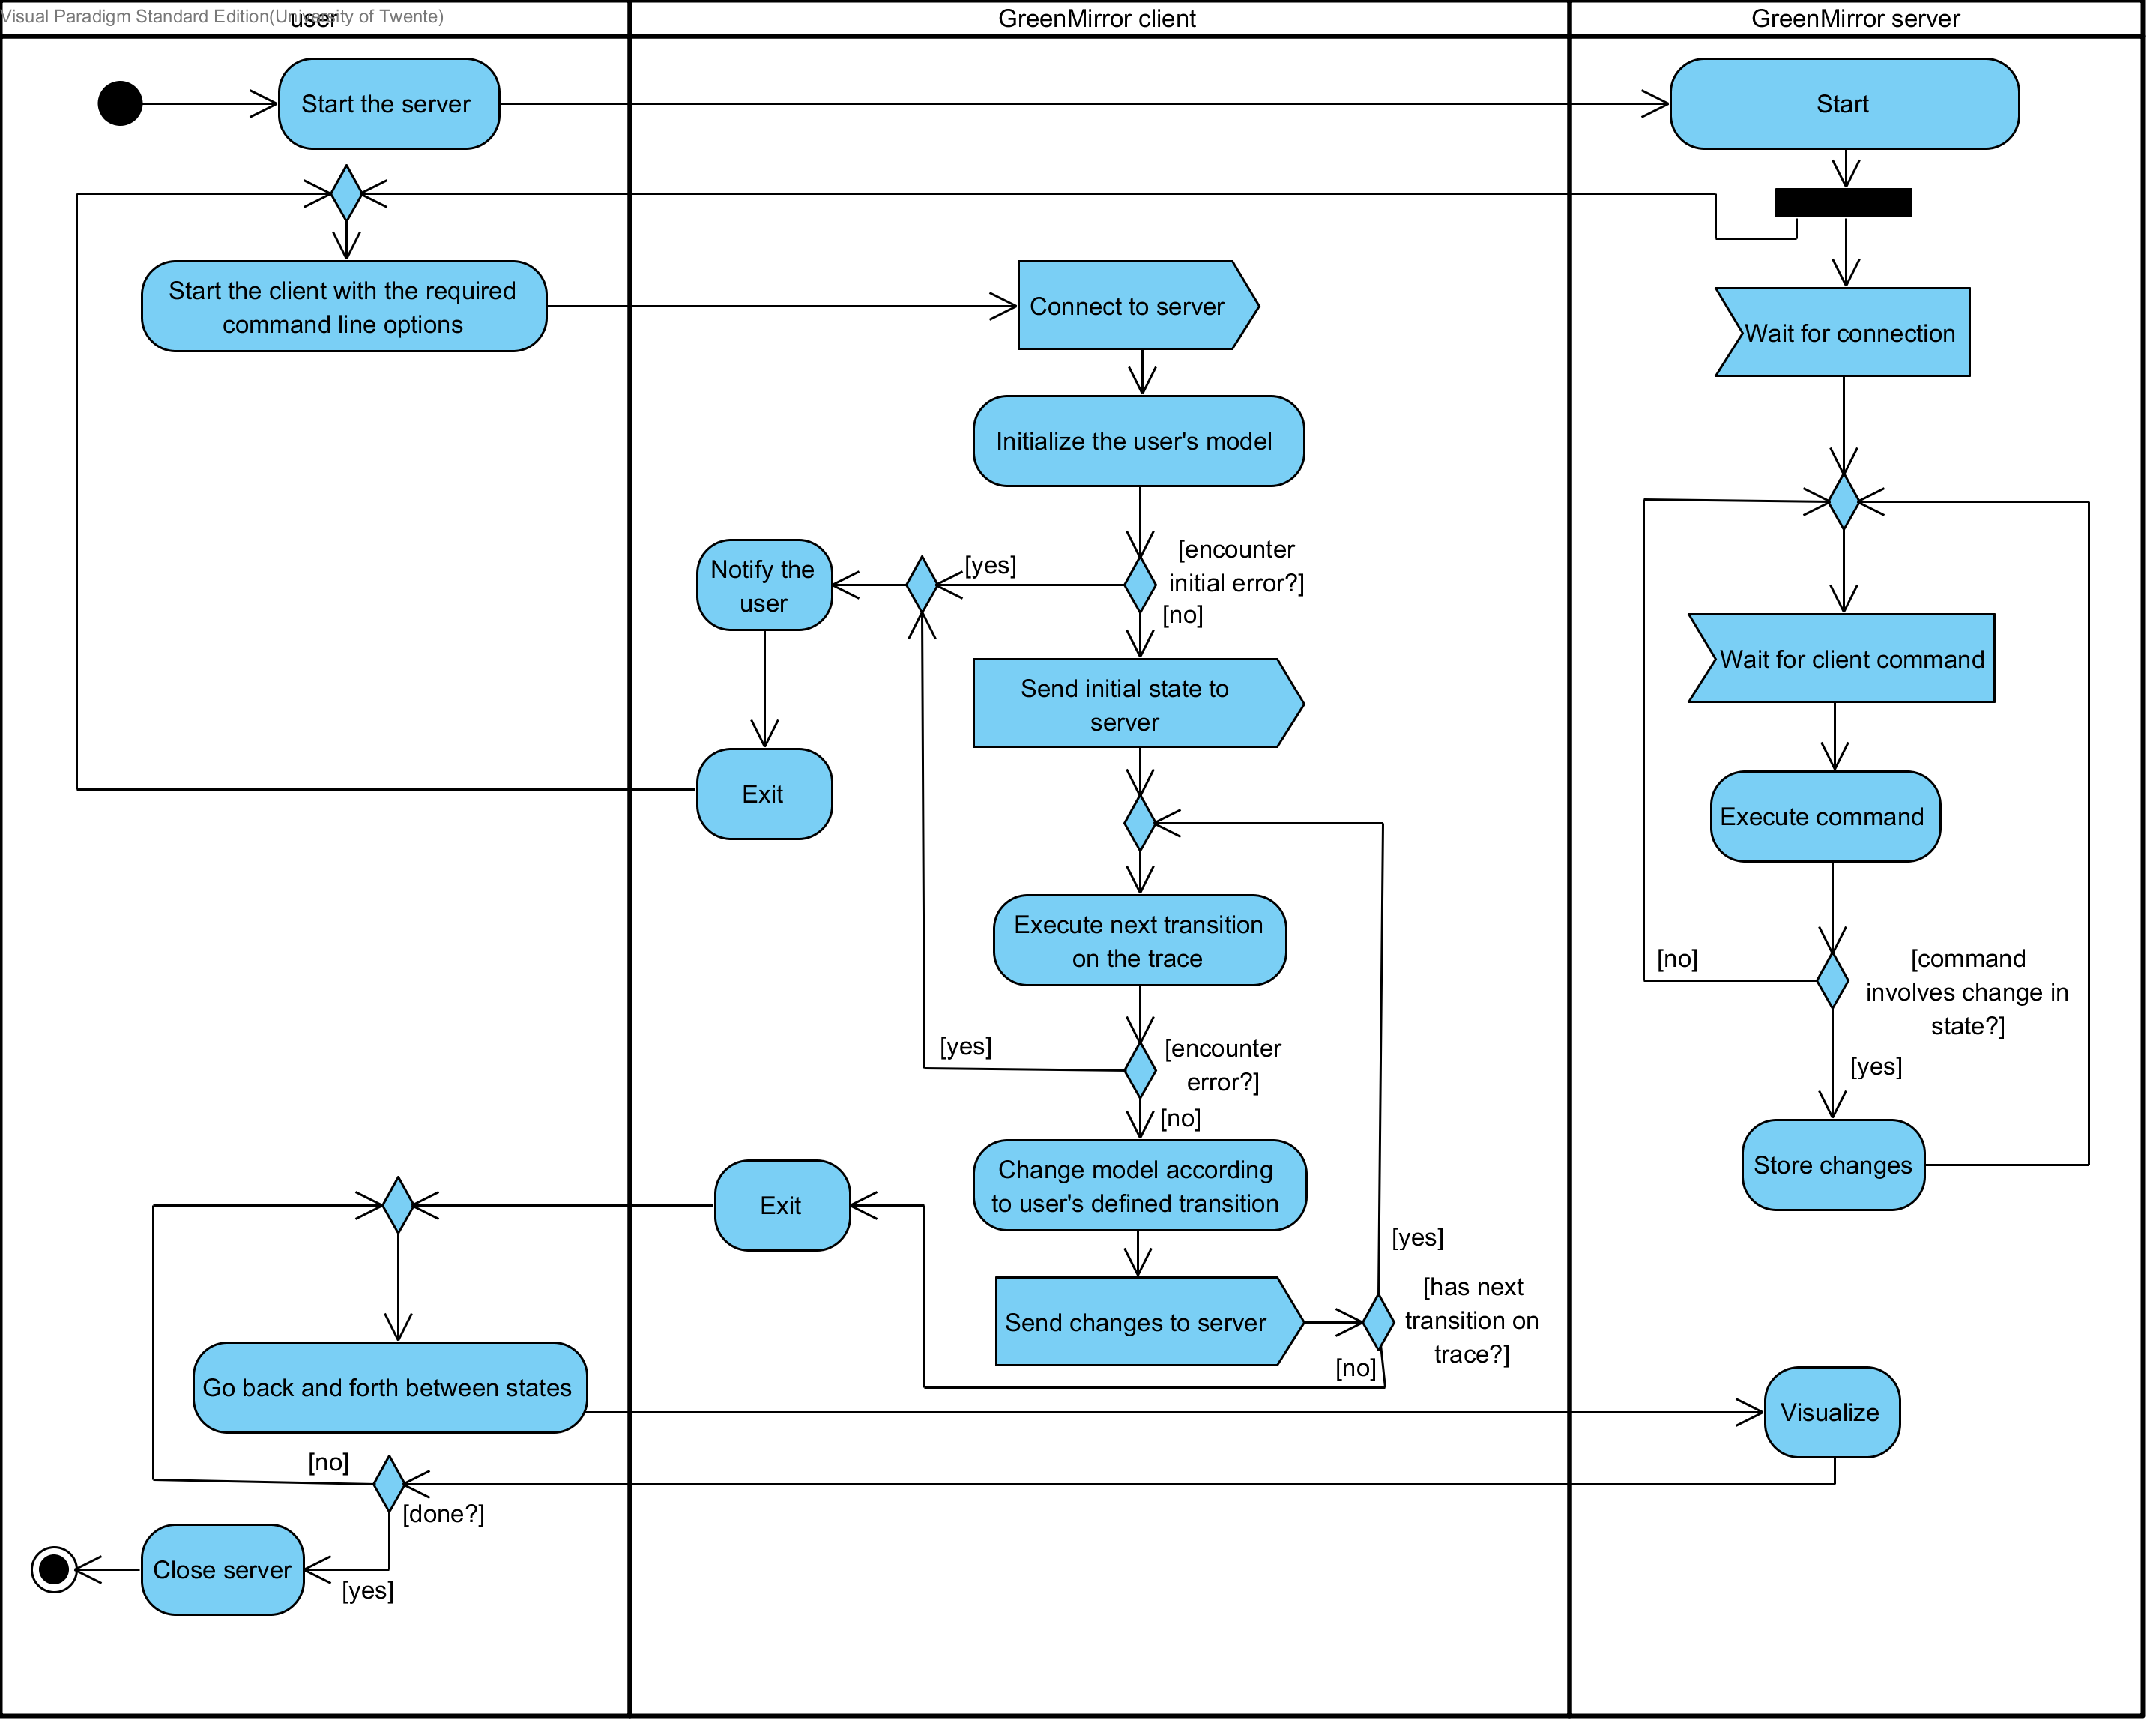
\includegraphics[width=1.0\textwidth]{diagrams/AD_generalworkflow}
  \caption{simplified activity diagram of the general work-flow}\label{fig:ad_generalworkflow}
\end{figure}
The general work-flow of a typical execution of the application is illustrated in the simplified activity diagram of \cref{fig:ad_generalworkflow}. This is meant to be fairly general: the exact work-flow depends on the used model initializers, the used trace selector and the user's model. In the current version, the visualization can only start when the whole model has been interpreted by the client and has been sent to the server. This behaviour is meant to ensure top performance while transitioning through the states, but can be easily modified.
%--------------------------------------------------------------------------------
\subsection{Detailed work-flow}\label{sec:design;sub:detailedwf}
The first thing that occurs when operating the application is starting up the client or server and parsing the command line options. GreenMirror uses the JOpt Simple library \cite{joptsimple} to parse command line options in the same way options can be used with executables of *nix operating systems. Available command line options implement the \lstinline{CommandLineOptionHandler} interface. This contains everything needed to handle options: option and argument specification, processing order, argument validation and option processing. See \cref{fig:sd_generalstartup} (\cref{app:seq}) for the (simplified) sequence of these events. From the diagram can be seen that the options are all validated before they are processed. This prevents partial processing without having all required and valid options (for example: initializing the model without a valid server address).\\
The importance of the validating, parsing and processing of command line options, however, should be explicitly stated. The complete set of the application's functions work as a direct consequence of the processing of these options. For example: the handler for the \lstinline{--host} option handles establishing the connection to the server and the handler for the \lstinline{--trace} option executes the trace. This results in the fact that new functionalities that should be executed during start-up can be easily added by implementing and adding new option handlers (see \cref{app:ext} for instructions).
\par\begin{wrapfigure}{r}{0.38\textwidth}\vspace{-20pt}
  \begin{center}
    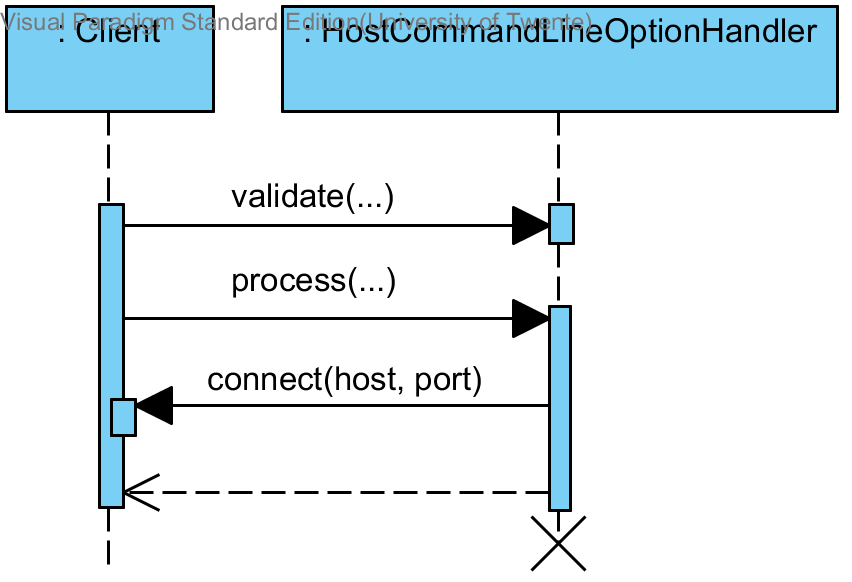
\includegraphics[width=0.36\textwidth]{diagrams/SD_client_host}
  \end{center}
  \vspace{-20pt}\caption{simplified sequence diagram of the handling of the \lstinline{--host} command line option}\vspace{-15pt}
  \label{fig:sd_client_host}
\end{wrapfigure}
Next are the implemented command line option handlers of the client. From here on out, the assumption is made that all required options are passed (\lstinline{--host}, \lstinline{--model} and \lstinline{--trace}) and that their arguments are valid. If that would not be the case, GreenMirror would have observed this before processing and would have notified the user before terminating, as is described in the previous paragraph. The first option that will be processed is the \lstinline{--host} option, which connects to the server. This is very straightforward and will requires no further elaboration. See \cref{fig:sd_client_host}.
\par Handling the model initializer option \lstinline{--model} is far more interesting. Several notable things are worth stating when looking at the sequence diagram in \cref{fig:sd_client_model} (\cref{app:seq}). Firstly, it can be seen that multiple model initializers can be selected. This is designed this way so the user can define the model in more than one way, perhaps even with the use of modules. In practise this can be used by simply passing the \lstinline{--model} option multiple times. Multiple model initializers are executed in the same order as they were passed via the command line. Secondly, a model initializer should define the model with the initial state and the state-transitions. The initial state can be defined by defining the initial nodes and relations and adding them to the controller. This sends the information directly to the server. Each state-transition is defined as an instance of the \lstinline{ModelTransition} class and holds a \lstinline{groovy.lang.Closure} field. This is code that is executed when the transition is executed and should transition the model to the next state. How the model initializer exactly defines the initial state and the state-transitions is up to the implementation (see \cref{sec:design;sub:interface}). Finally, when the model initializers have been executed and thus the initial state has been defined, GreenMirror sends the \lstinline{StartVisualization} command to the server, indicating that the transition to the first state can be performed. 
\par The \lstinline{--trace} option is handled next. See \cref{fig:sd_client_trace} (\cref{app:seq}) for the sequence diagram. This follows somewhat the same structure as the model initializer option handler, with a few slight differences. Only one \lstinline{TraceSelector} can be used. However, multiple \lstinline{ModelTransition}s can be executed with each transition from the trace, due to the fact that the \lstinline{ModelTransition} instance has a regular expression pattern that matches with zero to unlimited transitions from the trace. These transitions are executed in the order in which the model initializer added them to the controller. After each executed transition, GreenMirror sends an \lstinline{EndTransition} command to the server, indicating that a new state has been reached. If the user wants GreenMirror to refrain from sending this command, perhaps because the executed transition is part of the next one, the \lstinline{supplemental} flag of the \lstinline{ModelInitializer} instance can be set to \lstinline{true}.
\begin{figure}[ht]
  \centering
  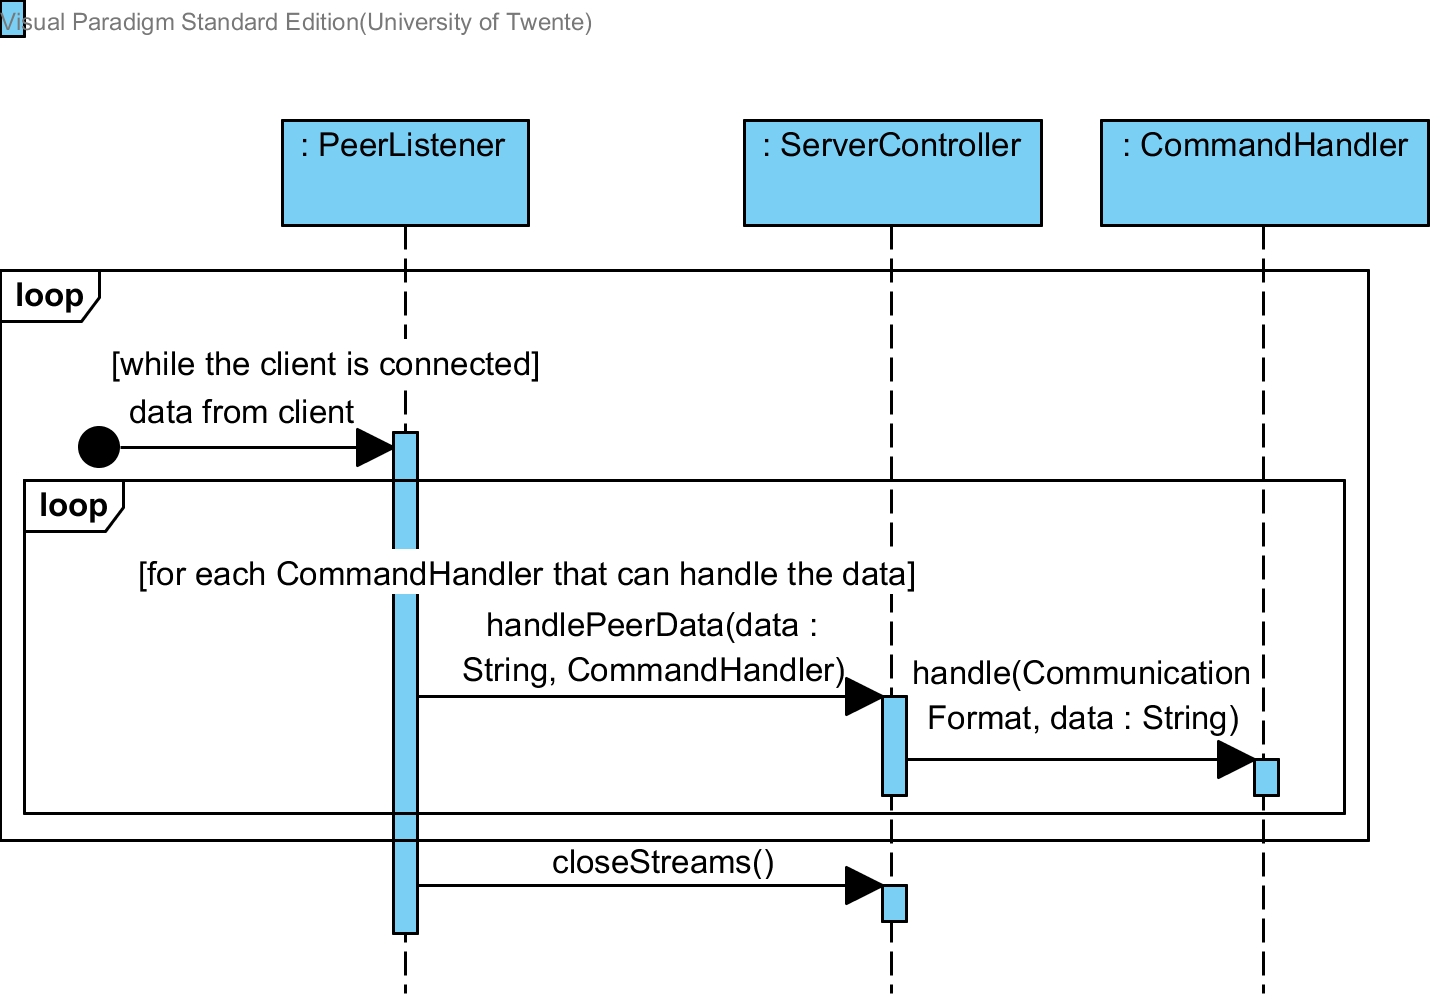
\includegraphics[width=0.6\textwidth]{diagrams/SD_server_receivecommand}
  \caption{simplified sequence diagram of the server receiving data}\label{fig:sd_server_receivecommand}
\end{figure}
\par The client is now finished and will close. In the meanwhile, the server has received the commands the client has sent. Every command is passed to the correct \lstinline{CommandHandler} in the sequence as shown in \cref{fig:sd_server_receivecommand}. What exactly happens in the \lstinline{handle(CommunicationFormat, String)} method of the \lstinline{CommandHandler} entirely depends on the received command.
\par After the client has sent the \lstinline{StartVisualization} command, the server starts the transition to the first state. Upon finishing, the correct toolbar buttons are enabled and the user can start interacting with the visualizer. What is seen in the sequence diagram of the user interaction (\cref{fig:sd_server_userinteraction} in \cref{app:seq}) is that all visualization parameters of the state-transition are derived from the button the user clicked on.
%More on this will be explained in \cref{subsec:implementationdetails}.
%TODO: check if the line above should be used (and the line above that).
%--------------------------------------------------------------------------------
\subsection{Interface design}\label{sec:design;sub:interface}
This section discusses the available interfaces for tool owners that provide ways of loading models into GreenMirror, and the current implementations. Loading a model consists of two parts: defining the model and providing the trace that defines in which order state-transitions will take place. Both parts have corresponding interfaces: respectively \lstinline{ModelInitializer} and \lstinline{TraceSelector}.
\par The model initializer has a few responsibilities. First and foremost it must, in the most general sense and not surprisingly, initialize the model according to the specifications of the user. More specifically: it must receive information from the user about how the initial state of the model is defined and how different state-transitions influence the model and the visualization. How the model initializer receives or retrieves this information is up to the implementation. Once it has received this information, it can add nodes to the client controller, remove nodes, add relations, etcetera. These changes are automatically conveyed to the server. The model initializer can also use the interface with the controller to send commands directly to the server, by use of the currently available commands in the \lstinline{greenmirror.commands} package. This behaviour is, however, not recommended, because this circumvents the logic incorporated in updating the model via the controller. It is meant to provide the possibility to send auxiliary commands such as the \lstinline{SetAnimationDuration} command.
\par The model initializers must define which state-transitions can happen by adding new instances of \lstinline{ModelTransition} to the controller. As mentioned in \cref{sec:design;sub:detailedwf}, this class has a \lstinline{groovy.lang.Closure} field that changes the model when the closure is executed. This type is chosen to directly support the first implemented model initializer, although it is not restricted to this first implementation. The closure can accept arguments based on the transitions on the trace. This is best explained using an example. Suppose the user wants to visualize a ConnectFour game. It would be unwieldy to define a state-transition for every possible move (although there are only seven at the most), so the user defines one state-transition that uses the regular expression \lstinline{^move([0-6])\$} to accept transitions from a trace. This means it needs the number of the column as an argument in the closure that executes the state-transition. Fortunately, the Groovy library supports this and GreenMirror takes advantage of this by supporting string and integer type arguments.
\par The server could be completely re-purposed by implementing different commands and command handlers. However, if the server is used as a visualizer, the model initializer has the responsibility of making sure the server first receives the initialization command. Without it, there is no JavaFX stage to which JavaFX nodes can be added. A tool owner developing a new model initializer could choose to delegate this responsibility to the user.
\par The model initializer that has been implemented in this first version of GreenMirror is based on Groovy \cite{groovy}. Groovy is a dynamic language for the Java platform and provides a vast array of useful features. Specifically, the model initializer uses Groovy's script functionalities. This choice was made due to the following reasons.
\begin{enumerate}
\item The user receives the power and flexibility of a full-featured programming language, but still is easy to learn. This means that both advanced programmers and users without much experience can use it.
\item The user scripts can be executed during runtime, meaning that, while employing a complete programming language, the GreenMirror framework doesn't have to be recompiled every time the user alters his model.
\item A clear interface with the controller can be provided to the user, which Groovy calls a \emph{base class}. The user can refer in his script to the base class' methods without referring to any object. This works as if the user is programming in the context of one of the methods of the base class (which it also comes down to, internally).
\end{enumerate}
\Cref{lst:groovyexample} shows an example of a user script that can be executed by the Groovy script model initializer. \Cref{fig:groovyexample} shows a screenshot of its resulting visualization. It can be seen from the listing that chained statements are possible and actually encouraged to improve the readability of the script. Another notable advantage is that it is easily seen that calls to the base class (and thus indirectly to the controller) indicate a read from or a write to the model. For example, creating a new \lstinline{Node} instance does not mean it is added to the model: \lstinline{addNodes()} takes care of that.
\lstinputlisting[label={lst:groovyexample}, caption={example Groovy script defining the user's state-transition model}]{code/example.java}
\begin{figure}[H]
  \centering
  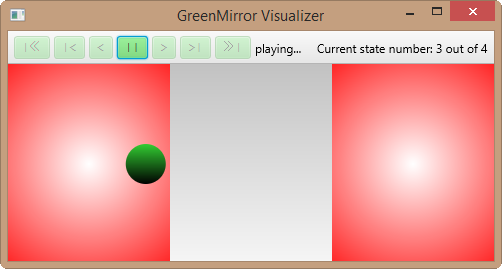
\includegraphics{images/groovyexample}
  \caption{a screenshot of the executing visualization of \cref{lst:groovyexample} with the trace from \cref{lst:traceexample}}\label{fig:groovyexample}
\end{figure}
\par After the model initializer has set the initial state and saved all \lstinline{ModelTransition}s, the selected \lstinline{TraceSelector} is executed. The current \lstinline{FileTraceSelector} implementation retrieves the trace from a text file where the transitions are separated by a newline. In the visualization example of \cref{fig:groovyexample}, the trace file looked like \cref{lst:traceexample}. In the toolbar of \cref{fig:groovyexample} a state count of four can be seen, while three transitions are in the trace. This is naturally because the initial state is included in the count.	
\begin{lstlisting}[label={lst:traceexample}, caption={example trace file for the model defined in \cref{lst:groovyexample}}]
switch
switch
switch
\end{lstlisting}
Both the \lstinline{ModelInitializer} and \lstinline{TraceSelector} interfaces accept one argument from the command line. This should be the source of the model and the trace, respectively. In \lstinline{GroovyScriptModelInitializer} it is the file name of the Groovy script, while in \lstinline{FileTraceSelector} it is the name of the file containing the trace. In future implementations that, for example, connect GreenMirror to another tool, this could be the name of the model.
%--------------------------------------------------------------------------------
\subsection{Implemented design patterns}\label{sec:design;sub:patterns}
GreenMirror conforms to several design patterns \cite{kuchana2004,sourcemaking} to stimulate future development and the overall maintainability of the framework. \Cref{tab:patterns} describes several implemented patterns, in alphabetical order. The name on the left side is the name of the design pattern. The right side describes the classes or structures that use the design pattern and contain information about the contexts in which the patterns are implemented.
\newpage\begin{longtable}{ |l p{10cm}| }
\caption{design patterns used in the GreenMirror framework}\label{tab:patterns}\\
\hline\multirow{2}{*}{\textbf{Builder}}
   & \texttt{GridBuilder} \\* & This class first accepts several required and optional parameters, after which it constructs the grid and finally returns the \texttt{NodeList} instance that contains the nodes that make up the grid. See \cref{sec:features;sub:gridbuilder} for more information and an example. \\
\hline\multirow{2}{*}{\textbf{Command}}
   & \texttt{Command} \\* & Whenever a subclass of \texttt{Command} is instantiated, the arguments are passed to its constructor. The \texttt{prepare()} method is called, in which the command can optionally execute preparations. Finally, the \texttt{getFormattedString(CommunicationFormat)} is called to retrieve a string that will be sent to the peer, formatted according to the parameter. \\
\hline \multirow{2}{*}{\textbf{Memento}}
   & states and state-transitions \\* & The memento pattern is specifically designed to store and retrieve the internal state of an object. This object is, in the case of GreenMirror, the visualizer. The internal state data is composed of the collection of JavaFX nodes and their properties, and the JavaFX transition data to progress to a next state. This pattern is implemented with the \texttt{Visualizer} and \texttt{VisualizerMemento} classes. Needless to say, \texttt{VisualizerMemento} fulfils the memento rule. The \texttt{Visualizer} class fulfils both the caretaker and originator roles, implementing the \texttt{VisualizerMemento.Caretaker} and \texttt{VisualizerMemento.Originator} interfaces to make this more expressive. It should be noted that the current version of GreenMirror only has need to store the JavaFX transition data in the memento. More on this will be explained in \cref{sec:design;sub:states}. \\
\hline\multirow{2}{*}{\textbf{Model-view-controller}}
   & \texttt{Node}, \texttt{Relation} - \texttt{Visualizer}, \texttt{Log} - \texttt{GreenMirrorController} \\* & GreenMirror uses the MVC pattern to improve maintainability. The model is represented by \texttt{Node} instances. If the user changes the model, the \texttt{Client} instance (which extends \texttt{GreenMirrorController}) is notified and in turn notifies \texttt{Log} and the server. The view and the model have no interaction whatsoever on the client's side. On the server's side, however, the controller role is shared by the \texttt{Visualizer} and \texttt{ServerController} instances because of the integrated functionalities. The view on the server's side is implemented by both \texttt{Visualizer} and \texttt{Log}, although it can also be argued that the server as a whole represents the view. \\
\hline\multirow{2}{*}{\textbf{Null object}}
   & \texttt{NullNode} \\* & Any GreenMirror node that gets removed in the user's model is replaced by an instance of \texttt{NullNode}. This makes sure the model throws expected exceptions and ensures the user will get properly notified if he tries to access it. \\
\hline\multirow{2}{*}{\textbf{Observer}}
   & \texttt{Node} \\* & The \texttt{Client} controller is notified of model updates, but only of nodes that have been added to the visualizer. \\
   & \texttt{FxWrapper} \\* & Every \texttt{Node} instance also is an observer: it observes any changes made in its FX. \\
\hline\multirow{2}{*}{\textbf{Prototype}}
   & \texttt{FxWrapper}, \texttt{Placement} \\* & All implemented subclasses are instantiated using the built-in \texttt{java.util.ServiceLoader} injector. When a new instance of \texttt{FxWrapper} or \texttt{Placement} is requested based on a data string, the string is compared to the stored instances and if a match is found, a clone of the matched instance is returned. \texttt{Placement} implementations can also be instantiated using the \texttt{new} operator, but both \texttt{FxWrapper} and \texttt{Placement} are at some point constructed via the prototype design pattern. \\
\hline\multirow{2}{*}{\textbf{Proxy}}
   & \texttt{FxWrapper} \\* & The \texttt{FxWrapper} class is exactly what the name says: a wrapper for the FX of a GreenMirror node. It generalizes handling the FX and provides intelligent access to certain FX properties. \\
   & \texttt{FxPropertyWrapper} \\* & The \texttt{FxPropertyWrapper} implementations primarily provide intelligent access to several methods that are often used. It is added to simplify adding support for different FX types and properties. \\
\hline\multirow{2}{*}{\textbf{State}}
   & \texttt{PlaybackState} \\* & The visualizer has a finite set of playback states it can be in. Certain things depend on the visualizer's playback state, such as which of toolbar buttons are enabled. The context role is taken up by the \texttt{Visualizer} instance, whereas the playback state is represented by instances of implementations of the \texttt{PlaybackState} class. \Cref{fig:smd_playbackstates} shows the state machine diagram belonging to the playback states. \\
\hline\multirow{2}{*}{\textbf{Strategy}}
   & \texttt{CommandHandler}, \texttt{CommandLineOptionHandler}, \texttt{FxWrapper}, \texttt{ModelInitializer}, \texttt{TraceSelector} \\* & All classes that implement the strategy design pattern do this so their subclasses can handle data in their own way. Which strategy (and thus which subclass of one of the above classes) is passed is determined at runtime. For example: every \texttt{ModelInitializer} implementation has its own \texttt{executeInitializer()} method that initializes the user's model in its own way. Which \texttt{ModelInitializer} is executed, depends on which the user selects during runtime. The \texttt{Log} class also uses this pattern, only it accepts \texttt{PrintStream} subclasses as strategies. \\
\hline
\end{longtable}
\begin{figure}[h]
  \centering
  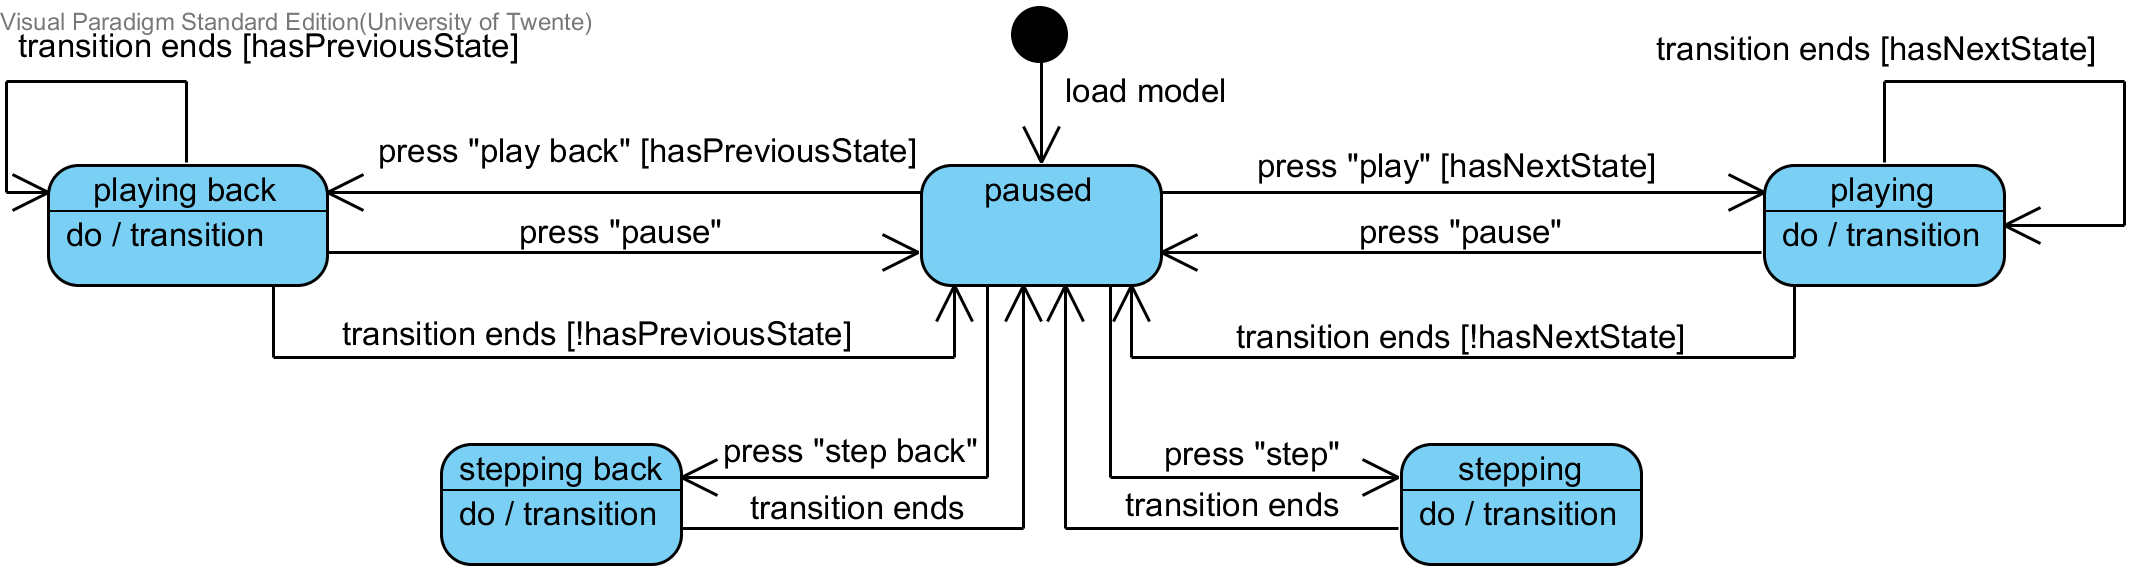
\includegraphics[width=\textwidth]{diagrams/smd_playbackstates}
  \caption{the state machine diagram for the visualizer's playback states}\label{fig:smd_playbackstates}
\end{figure}
%--------------------------------------------------------------------------------
\subsection{Internal representation of visual node properties}\label{sec:design;sub:fxwrapper}
The \lstinline{FxWrapper} class and its subclasses store and track the FX properties of GreenMirror nodes, as is explained in \cref{sec:features;sub:nodrel}. Using a wrapper instead of directly using a JavaFX node instance has the following reasons.
\begin{enumerate}
\item \lstinline{FxWrapper} provides general methods such as converting FX data into an object that can be shared between client and server, or changing general properties like the rotation and opacity of a JavaFX node.
\item The implementations of abstract methods of \lstinline{FxWrapper} used by GreenMirror might differ per type of JavaFX node. For example: the calculations of a specific placement on the edge of a circle differ from the calculations of a placement on the edge of a rectangle.
\item For the logic in the user's model and the proper creation of state-transitions on the server, properties have to be set and changed during the processing of state-transitions in the model without directly affecting the FX in the visualizer. As will be explained in \cref{sec:design;sub:states}, changing actual properties of JavaFX nodes happens as a consequence of the execution of JavaFX transitions. To work with these values without directly visualizing them, a wrapping layer is needed providing 'virtual' values. 
\item Support for new types of JavaFX nodes can be easily added. Examples include ellipses, three-dimensional shapes and composite nodes.
\end{enumerate}
The way \lstinline{FxWrapper} converts its properties to an object that can be sent over the network, is generalized in the sense that support for new types of properties can also be implemented easily. The following example will clarify this. One of the supported properties of \lstinline{ImageFxWrapper} is the X coordinate of type \lstinline{double}. In the current GreenMirror version, FX data is sent to the server in JSON format (see \cref{sec:design;sub:interchange}). The value of the X coordinate can be easily converted to and from a string format, as would the \lstinline{boolean}-type \lstinline{preserveRatio} property. So how would the \lstinline{image} property of type \lstinline{javafx.scene.image.Image} be converted to and from a valid JSON string? The implementations of \lstinline{FxPropertyWrapper} handle the FX properties to make this modular and easily extensible. In the case of the example about the image, the \lstinline{ImageFxProperty} class handles the \lstinline{image} property.
%--------------------------------------------------------------------------------
\subsection{Internal representation of states and state-transitions}\label{sec:design;sub:states}
\begin{wrapfigure}{o}{0.38\textwidth}\vspace{-20pt}
\begin{center}
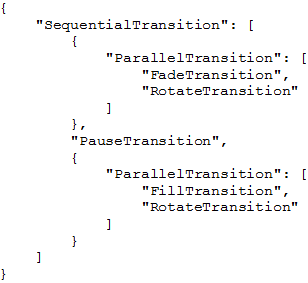
\includegraphics[width=0.36\textwidth]{diagrams/transitiontree}
\end{center}
\vspace{-10pt}\caption{an example of one stored state-transition in JSON notation}\vspace{-12pt}
\label{fig:transitiontree}
\end{wrapfigure}
State data is not stored in the current version of GreenMirror, because it is unnecessary. To understand why this is, an explanation must be provided about how state-transition data is stored and how JavaFX handles its transitions (animations, in this case).
\par GreenMirror uses classes that extend \lstinline{javafx.animation.Transition}. These classes hold all data needed to perform an animation: start and end value of an FX property and a method that handles the temporal behaviour of the value. JavaFX also provides two special transition implementations: \lstinline{ParallelTransition} and \lstinline{SequentialTransition}. These handle other transitions that are added to their lists in parallel or sequentially, respectively, and can be nested.
This is also how GreenMirror stores a state-transition: one \lstinline{SequentialTransition} instance holding one or multiple \lstinline{ParallelTransition} instances (separated by a \lstinline{PauseTransition} to incorporate an optional delay) which in turn hold the individual \lstinline{Transition} instances that animate the change in properties. Initially, every change in the model the server receives ends up in the same top-level \lstinline{ParallelTransition}. The user might want to show several sequential animations during one state-transition. For this scenario, the flush command has been implemented. This results in the server creating a new \lstinline{ParallelTransition} instance in the root \lstinline{SequentialTransition} in which all further transitions will be stored. For an example of these nested transitions of one state-transition, see \cref{fig:transitiontree}. JavaFX' transition classes also have another interesting functionality: the \lstinline{rate} property. When set to a negative value, the animation reverses. This makes browsing backwards through the model's states very easy and removes the need to recalculate FX property values of JavaFX nodes.
\par These reasons make storing state data unnecessary. State-transition data is composed of the JavaFX animations needed to go from one state to another, including the start and end values of the relevant FX properties, whichever direction the user wants to go.
%--------------------------------------------------------------------------------
\subsection{Interchange formats}\label{sec:design;sub:interchange}
Nothing is currently being stored of the result of a visualization. The formats associated with defining the user's model and the corresponding trace are discussed in \cref{sec:design;sub:interface}. This leaves the protocol used between the client and the server. This is very simple and has the form \texttt{command:commanddata}. The part before the colon holds the name of the command as it is presented in \cref{sec:features;sub:commands}. This is included so the receiver knows which \lstinline{CommandHandler} implementation can handle the command data. The part after the colon holds the command data, formatted in the selected \lstinline{CommunicationFormat}. The JSON format is currently the only supported format. An example of a command is shown in \cref{lst:commandexample}.
\begin{lstlisting}[label={lst:commandexample}, caption={an example command sent from the client to the server in the JSON communication format, indicating that a node as been added to the model}]
AddNode:{"id":2,"identifier":"nodetype:nodename"}
\end{lstlisting}